\documentclass[12pt,a4paper]{article}
\usepackage[T1,T2A]{fontenc}
\usepackage[utf8]{inputenc}
\usepackage[english,russian]{babel}
\usepackage{microtype}
\usepackage{csquotes}
\usepackage{amsmath}
\usepackage{amsthm}
\usepackage{amssymb}
\usepackage{mathtext}
\usepackage[notrig,italicdiff]{physics}
\usepackage{newfloat}
\usepackage{caption}
\usepackage{indentfirst}
\usepackage{geometry}
\usepackage{hyperref}
\usepackage{mdframed}
\usepackage[inline]{enumitem}
\usepackage{graphicx}
\usepackage{subfig}
\usepackage{titlesec,titletoc}
\usepackage[titletoc,title]{appendix}
\geometry{left=3cm,right=2cm,top=2cm,bottom=2cm}
\DeclareGraphicsExtensions{.pdf,.png,.jpg,.PNG}
\graphicspath{{./img/}}
\captionsetup[figure]{justification=centering}
\renewcommand{\thesubfigure}{\asbuk{subfigure}}
\DeclareCaptionLabelSeparator{dotseparator}{. }
\titlelabel{\thetitle. }
\patchcmd{\appendices}{\quad}{. }{}{}
\captionsetup{labelsep=dotseparator}
\hypersetup{
	colorlinks,
	citecolor=black,
	filecolor=black,
	linkcolor=black,
	urlcolor=black
}

\begin{document}

    \newcommand\blanktextfield[2]{$\underset{\text{#1}}{\text{\underline{\hspace{#2}}}}$}

\makeatletter
\begin{titlepage}

	\large\newpage

    \noindent\centering{
    	МИНИСТЕРСТВО ОБРАЗОВАНИЯ И НАУКИ РОССИЙСКОЙ ФЕДЕРАЦИИ

    	Федеральное государственное автономное образовательное учреждение высшего образования \enquote{Национальный исследовательский Нижегородский государственный университет им. Н.И. Лобачевского}
    }

	\vspace*{50pt}

	Физический факультет \\[\baselineskip]

	Кафедра информационных технологий\\
	в физических исследованиях

	\vspace*{\fill}

	{\Large\textbf{Сжатие-восстановление изображения (архивация) методом, аналогичным JPEG}}

	\vspace*{\fill}

	\hfill\begin{minipage}{22em}
    	Отчет по учебной практике\\
		студента 1 курса магистратуры 05182 группы\\
		\textbf{Василевского А.В.}
    \end{minipage} \\[\baselineskip]

	\hfill\begin{minipage}{22em}
		Основная профессиональная образовательная
		программа подготовки магистров по
		направлению 09.04.02~--- \enquote{Информационные системы и технологии}
		(профиль программы: \enquote{Информационные системы и технологии в физических исследованиях})
    \end{minipage}

	\vspace*{\fill}

	\hfill\begin{minipage}{15em}
		\blanktextfield{(подпись)}{1in} Василевский А.В.\\[\baselineskip]
		Руководитель:\\
		проф. кафедры ИТФИ\\
		к. ф.-м. н.\\[\baselineskip]
		\blanktextfield{(подпись)}{1in} Морозов О.А.
    \end{minipage}

	\vspace*{\fill}

	Нижний Новгород\\
	2018

\end{titlepage}
\makeatother


    \tableofcontents

    \clearpage

    %
    %
    %
    %%%%%%%%%%%%%%%%%%%%%%%%%%%%%%%%%%%%%%%%%%%%%%%%%%%%%%%%%%%%%%%%%%%%%%%
    %                           SECTION                                   %
    %%%%%%%%%%%%%%%%%%%%%%%%%%%%%%%%%%%%%%%%%%%%%%%%%%%%%%%%%%%%%%%%%%%%%%%
    %
    %
    %

    \section{Постановка задачи}

        Изучить основы сжатия и восстановления изображения методом JPEG. Получить базовое представление о принципах сжатия изображений с потерями. Исследовать качество сжатия и восстановления различных типов изображений в зависимости от параметра степени сжатия.

    %
    %
    %
    %%%%%%%%%%%%%%%%%%%%%%%%%%%%%%%%%%%%%%%%%%%%%%%%%%%%%%%%%%%%%%%%%%%%%%%
    %                           SECTION                                   %
    %%%%%%%%%%%%%%%%%%%%%%%%%%%%%%%%%%%%%%%%%%%%%%%%%%%%%%%%%%%%%%%%%%%%%%%
    %
    %
    %

    \section{Теоретическая часть}

        %
        %
        %
        %%%%%%%%%%%%%%%%%%%%%%%%%%%%%%%%%%%%%%%%%%%%%%%%%%%%%%%%%%%%%%%%%%%
        %                        SUBSECTION                               %
        %%%%%%%%%%%%%%%%%%%%%%%%%%%%%%%%%%%%%%%%%%%%%%%%%%%%%%%%%%%%%%%%%%%
        %
        %
        %

        \subsection{Алгоритм JPEG}

            Алгоритм JPEG (Joint Photographic Experts Group)~--- один из алгоритмов сжатия изображений с потерями. В основе метода лежит тот факт, что человеческое зрение плохо различает близкие оттенки цвета и близкие уровни яркости. Таким образом, отбрасывая несущественную для восприятия человека информацию, алгоритм JPEG обеспечивает высокую степень сжатия при относительно низкой (управляемой) степени потери качества. JPEG подходит в основном для сжатия фотографических изображений с большим количеством градаций цвета и преобладанием низких пространственных частот.

            Стандарт JPEG очень сложный, предусматривает как сжатие с потерями, так и без потерь, поддержку прогрессивного сжатия, когда окончательное изображение строится из нескольких \enquote{слоев}, постепенно \enquote{уточняющих} друг друга и т.д. Мы не будем описывать весь стандарт или какую-то его часть, а рассмотрим общий принцип, лежащий в основе метода.

            Сжатие по JPEG производится в несколько этапов. Далее мы рассмотрим некоторые этапы в отдельности более подробно.
            %
            \begin{enumerate}
                \item \textbf{Дискретизация}. Производится перевод RGB-изображения в цветовое пространство YCbCr и его субдискретизация (квантование).
                \item \textbf{Косинусное преобразование}. Изображение делится на области $8\times 8$ пикселей и над каждой областью в отдельности выполняется двумерное дискретное косинусное преобразование.
                \item \textbf{Квантование}. На этом этапе отбрасываются несущественные коэффициенты косинусного преобразования. В этом заключается основа сжатия по методу JPEG.
                \item \textbf{Сжатие без потерь}. Над оставшимися коэффициентами производится сжатие по методу RLE (Run Length Encoding), после чего применяется кодирование по Хаффману.
            \end{enumerate}
            %
            Как уже было отмечено, основное сжатие изображения происходит на этапе квантования. Этап сжатия без потерь является важным, хотя и дополнительным действием. В рамках данного теоретического изложения мы его опустим.

            Декодирование (восстановление) изображения производится аналогично в обратном порядке.

        %
        %
        %
        %%%%%%%%%%%%%%%%%%%%%%%%%%%%%%%%%%%%%%%%%%%%%%%%%%%%%%%%%%%%%%%%%%%
        %                        SUBSECTION                               %
        %%%%%%%%%%%%%%%%%%%%%%%%%%%%%%%%%%%%%%%%%%%%%%%%%%%%%%%%%%%%%%%%%%%
        %
        %
        %

        \subsection{Дискретизация}

            Человеческое зрение лучше различает близкие значения яркости, чем близкие значения оттенка цвета. Отсюда возникает идея кодировать яркостную компоненту отдельно от компонент цветности и сжимать ее менее агрессивно.

            Именно эту цель и преследует этап дискретизации. Цветовое пространство RGB не содержит выделенного канала яркости, а все три основных цвета входят в него равноправно. Пространство YCbCr отделяет компоненту яркости от компонент цветности, позволяя сжимать их независимо.

            Преобразование вектора цвета при переходе от RGB к YCbCr сводится к линейным операциями. Формулы данного перехода могут быть найдены в [\cite{miano_jpeg}].

            На данном этапе может быть выполнена субдискретизация компонент вектора цвета с различным шагом для яркостной компоненты и компонент цветности.

        %
        %
        %
        %%%%%%%%%%%%%%%%%%%%%%%%%%%%%%%%%%%%%%%%%%%%%%%%%%%%%%%%%%%%%%%%%%%
        %                        SUBSECTION                               %
        %%%%%%%%%%%%%%%%%%%%%%%%%%%%%%%%%%%%%%%%%%%%%%%%%%%%%%%%%%%%%%%%%%%
        %
        %
        %

        \subsection{Косинусное преобразование}

            Косинусное преобразование~--- вариант преобразования Фурье для симметричного сигнала. Одно из главных его достоинств в приложении сжатию изображений~--- действительность коэффициентов преобразования для действительного сигнала.

            Косинусное преобразование выполняется независимо над областями изображения размером $8\times 8$ пикселей отдельно для каждой цветовой компоненты.

            Дискретное двумерное косинусное преобразование для такого блока определяется следующей формулой:
            %
            \begin{equation*}
                S'[i,j]=\sum\limits_{x=0}^{N-1}\sum\limits_{y=0}^{N-1}c[i,j]S[y,x]\cos{\frac{(2y+1)i\pi}{2N}}\cos{\frac{(2x+1)j\pi}{2N}},
            \end{equation*}
            %
            где $S[x,y]$~--- исходное изображение, $S'[i,j]$~--- его образ (преобразование),
            %
            \begin{equation*}
                c[i,j]=\frac{(\delta[i,j]+1)}{N}, \quad \delta[i,i] = 1, \quad \delta[i,j] = 0 .
            \end{equation*}
            %
            При этом $S$ и $S'$ равноправны, т.е. указанное преобразование сохраняет форму при замене $S$ на $S'$.

            При реализации алгоритма на компьютере следует помнить, что коэффициенты косинусного преобразования вообще говоря не являются неотрицательными (в отличие от компонент вектора цвета).

        %
        %
        %
        %%%%%%%%%%%%%%%%%%%%%%%%%%%%%%%%%%%%%%%%%%%%%%%%%%%%%%%%%%%%%%%%%%%
        %                        SUBSECTION                               %
        %%%%%%%%%%%%%%%%%%%%%%%%%%%%%%%%%%%%%%%%%%%%%%%%%%%%%%%%%%%%%%%%%%%
        %
        %
        %

        \subsection{Квантование}

            Квантование служит для уменьшения количества информации, приходящейся на один коэффициент преобразования, а также устранения коэффициентов, соответствующих высоким пространственным частотам.

            Оно осуществляется (прямым покомпонентным) делением матрицы коэффициентов преобразования на матрицу квантования и последующим взятием целой части. Вариант матрицы квантования (\enquote{стандартной} матрицы квантования) представлен в стандарте JPEG [\cite{ccitt_jpeg},\cite{mitchell_jpeg}]. Ее коэффициенты подбираются с той целью, чтобы уменьшить количество информации, приходящееся на высокочастотные компоненты, а также уменьшить общее количество информации, приходящееся на все компоненты, т.е. произвести частотно-зависимое квантование коэффициентов косинусного преобразования. В основном коэффициенты такой матрицы увеличиваются с увеличением номера строки или столбца: минимальны в верхнем левом углу и максимальны в нижнем правом.

            Для различных компонент вектора цвета могут применяться разные матрицы квантования. Так, стандарт определяет вариант матрицы для яркостного канала и отдельный вариант матрицы для каналов цветности.

            По окончании процесса квантования результирующие коэффициенты преобразования являются малыми по величине целыми числами. При этом в области высоких частот образуется много нулевых коэффициентов. Поэтому в стандарте предусмотрено сжатие без потерь, служащее для оптимизации последовательностей одинаковых и малых по величине чисел.

            При декодировании соответствующие коэффициенты квантованной матрицы коэффициентов преобразования умножаются на коэффициенты матрицы квантования.

    %
    %
    %
    %%%%%%%%%%%%%%%%%%%%%%%%%%%%%%%%%%%%%%%%%%%%%%%%%%%%%%%%%%%%%%%%%%%%%%%
    %                           SECTION                                   %
    %%%%%%%%%%%%%%%%%%%%%%%%%%%%%%%%%%%%%%%%%%%%%%%%%%%%%%%%%%%%%%%%%%%%%%%
    %
    %
    %

    \section{Практическая часть}

        %
        %
        %
        %%%%%%%%%%%%%%%%%%%%%%%%%%%%%%%%%%%%%%%%%%%%%%%%%%%%%%%%%%%%%%%%%%%
        %                        SUBSECTION                               %
        %%%%%%%%%%%%%%%%%%%%%%%%%%%%%%%%%%%%%%%%%%%%%%%%%%%%%%%%%%%%%%%%%%%
        %
        %
        %

        \subsection{Управление качеством}

            Хотя спецификация JPEG покрывает множество аспектов его применения, тема управления качеством сжатия раскрыта слабо. Чтобы восполнить этот недостаток и продемонстрировать возможность управления потерями при сжатии приведем здесь простую схему, построенную на тех же элементарных соображениях, что и матрица квантования.

            Наиболее простое решение состоит в умножении матрицы квантования на некоторый коэффициент, зависящий от параметра качества. Если принять \enquote{качество}, стандартной матрицы квантования за $0.5$ и обратить внимание на то, что значение коэффициентов в матрице ограничены сверху значением $M$~--- верхней границей диапазона изменения коэффициентов косинусного преобразования (в силу операции взятия целой части при квантовании), можно получить формулу вида:
            %
            \begin{equation*}
                k = M - 2 (M - 1) q,
            \end{equation*}
            %
            где $k$~--- множитель матрицы квантования, $q$~--- показатель качества ($0-0.5$).

            Следует отметить, что младший коэффициент матрицы квантования лучше подвергнуть минимальным изменениям, поскольку он определяет фоновую яркость и цветность всего блока $8\times 8$.

        %
        %
        %
        %%%%%%%%%%%%%%%%%%%%%%%%%%%%%%%%%%%%%%%%%%%%%%%%%%%%%%%%%%%%%%%%%%%
        %                        SUBSECTION                               %
        %%%%%%%%%%%%%%%%%%%%%%%%%%%%%%%%%%%%%%%%%%%%%%%%%%%%%%%%%%%%%%%%%%%
        %
        %
        %

        \subsection{Описание демонстрационной программы}

            В ходе работы была разработана программа на языке $C++$ (\autoref{fig:mainwindow}), позволяющая визуально и численно исследовать качество и степень сжатия изображения по принципу метода JPEG. Программа позволяет задать фиксированную степень сжатия и оценить среднеквадратичное отклонение восстановленного изображения от оригинального и отношение размера сжатого изображения к размеру несжатого. А также увидеть зависимость этих параметров от параметра степени сжатия.
            %
            \begin{figure}[!htb]%
                \centering
                %
                \subfloat[][]{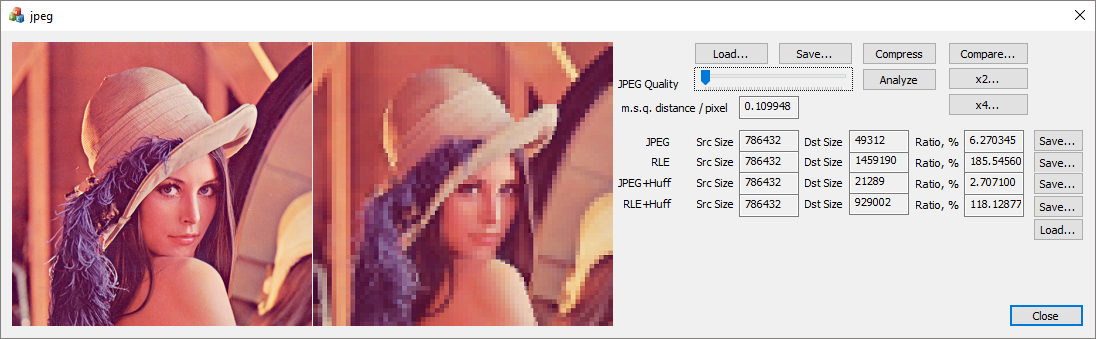
\includegraphics[width=0.8\textwidth]{mainwindow}}%
                \hspace{8pt}%
                %
                \caption[]{Главное окно программы.}%
                \label{fig:mainwindow}%
            \end{figure}

            В программе помимо базового JPEG-сжатия реализовано также и сжатие без потерь (как часть JPEG-сжатия и как самостоятельный алгоритм). Это позволит судить о том, какие классы изображений JPEG сжимает лучше.

        %
        %
        %
        %%%%%%%%%%%%%%%%%%%%%%%%%%%%%%%%%%%%%%%%%%%%%%%%%%%%%%%%%%%%%%%%%%%
        %                        SUBSECTION                               %
        %%%%%%%%%%%%%%%%%%%%%%%%%%%%%%%%%%%%%%%%%%%%%%%%%%%%%%%%%%%%%%%%%%%
        %
        %
        %

        \subsection{Анализ результатов}

            На \autoref{fig:1} можно видеть оригинальное и сжатое методом JPEG изображение класса \enquote{фотография}. Видно, что с увеличением степени сжатия изображение все более становится \enquote{пиксельным}. Это свидетельствует о том, что в блоках $8\times 8$ с увеличением степени сжатия остается все меньше и меньше высоких частот. Следует отметить, что хоть качество изображения и снизилось, фактически все \enquote{важные} детали сохранены.
            %
            \begin{figure}[!htb]%
                \centering
                %
                \subfloat[][]{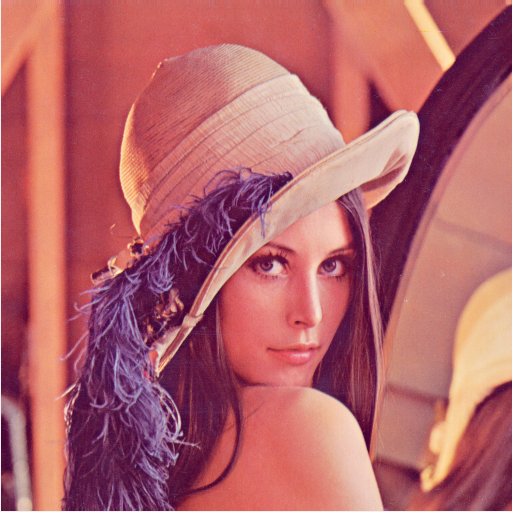
\includegraphics[width=0.4\textwidth]{lenna100}}%
                \hspace{8pt}%
                %
                \subfloat[][]{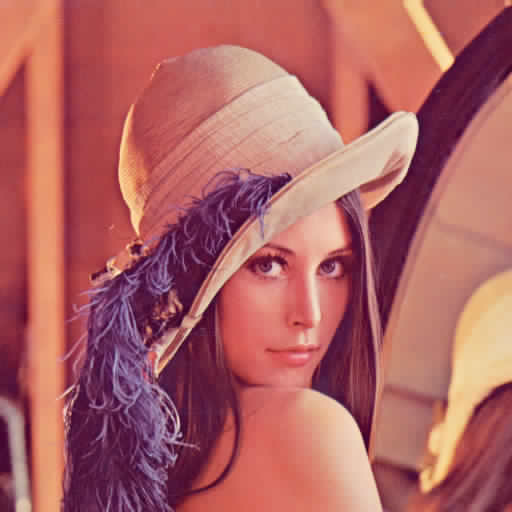
\includegraphics[width=0.4\textwidth]{lenna50}}%
                \hspace{8pt}%
                %
                \subfloat[][]{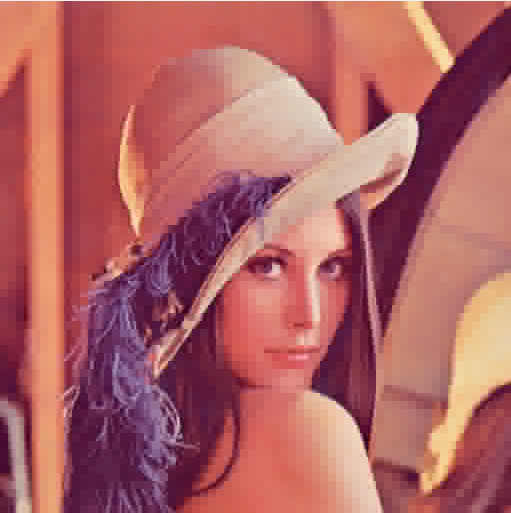
\includegraphics[width=0.4\textwidth]{lenna35}}%
                \hspace{8pt}%
                %
                \subfloat[][]{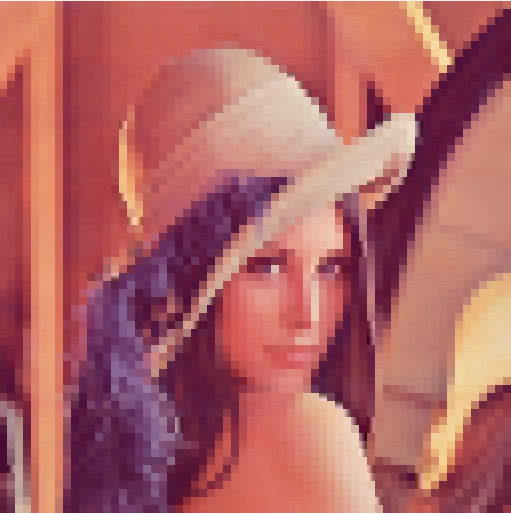
\includegraphics[width=0.4\textwidth]{lenna0}}%
                \hspace{8pt}%
                %
                \caption[]{Оригинальная и сжатые фотографии с разными показателями степени сжатия ($q=0.5,0.35,0$).}%
                \label{fig:1}%
            \end{figure}

            Сжатие по JPEG данной фотографии оставляет лишь $6-8$\% ($2-4$\% при дополнительном сжатии без потерь) от размера исходного изображения, в то время как сжатие без потерь лишь достигает уровня $80$\%.

            Если мы рассмотрим другой класс изображений (\autoref{fig:2}), а именно класс \enquote{рисунков}, мы увидим, что при том же уровне сжатия JPEG сжатие без потерь от него не отстает, а при большом размере исходного изображения может даже показать более высокий уровень сжатия. Это связано с тем, что рисованные изображения (мультфильмы) содержат большое количество однородных по цвету областей, которые прекрасно сжимаются алгоритмами сжатия без потерь. Кроме того, в рисованных изображениях важны мелкие детали, как то линии контуров, которые JPEG \enquote{размазывает} по блокам. Вокруг тонких линий появляются артефакты сжатия~--- \enquote{дублирующие} линии. Таким образом, рисованные изображения JPEG визуально искажает сильнее.
            %
            \begin{figure}[!htb]%
                \centering
                %
                \subfloat[][]{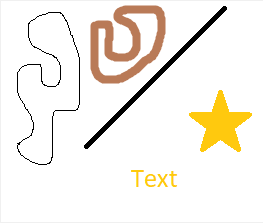
\includegraphics[width=0.4\textwidth]{curves100}}%
                \hspace{8pt}%
                %
                \subfloat[][]{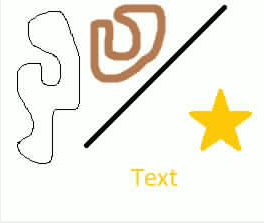
\includegraphics[width=0.4\textwidth]{curves50}}%
                \hspace{8pt}%
                %
                \subfloat[][]{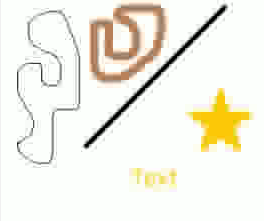
\includegraphics[width=0.4\textwidth]{curves35}}%
                \hspace{8pt}%
                %
                \subfloat[][]{
\includegraphics[width=0.4\textwidth]{curves0}}%
                \hspace{8pt}%
                %
                \caption[]{Оригинальная и сжатые рисунки с разными показателями степени сжатия ($q=0.5,0.35,0$).}%
                \label{fig:2}%
            \end{figure}

            Взглянем теперь на графики зависимости уровня сжатия и качества восстановления от параметра степени сжатия (\autoref{fig:3}). Общей тенденцией является монотонный нелинейный характер поведения уровня сжатия и качества восстановления изображения. Нелинейность связана также с выбором метода управления качеством. Также можно видеть, что степень сжатия более круто меняет свое значение при высоком параметре качества, в то время как кривая качества восстановления более полога. Это говорит о том, что уменьшение параметра качества слабо влияет на сжатие, в то же время вызывая сильное изменение качества восстановления изображения.
            %
            \begin{figure}[!htb]%
                \centering
                %
                \subfloat[][]{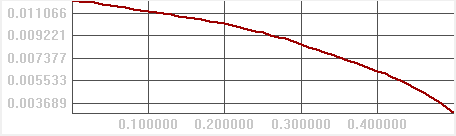
\includegraphics[width=0.4\textwidth]{lennaplt}}%
                \hspace{8pt}%
                %
                \subfloat[][]{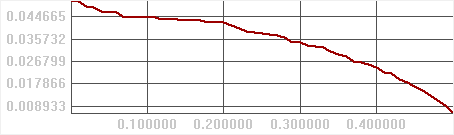
\includegraphics[width=0.4\textwidth]{curvesplt}}%
                \hspace{8pt}%
                %
                \subfloat[][]{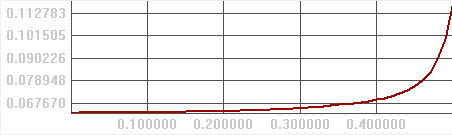
\includegraphics[width=0.4\textwidth]{lennapltc}}%
                \hspace{8pt}%
                %
                \subfloat[][]{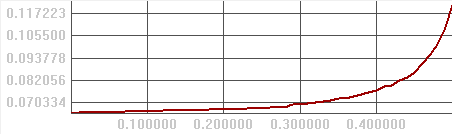
\includegraphics[width=0.4\textwidth]{curvespltc}}%
                \hspace{8pt}%
                %
                \caption[]{Зависимость качества восстановления (сверху) и степени сжатия (снизу) от показателя уровня сжатия $q$ для фотографического изображения (справа) и рисунка (слева). По горизонтальной оси отложен показатель $q$.}%
                \label{fig:3}%
            \end{figure}

    %
    %
    %
    %%%%%%%%%%%%%%%%%%%%%%%%%%%%%%%%%%%%%%%%%%%%%%%%%%%%%%%%%%%%%%%%%%%%%%%
    %                           SECTION                                   %
    %%%%%%%%%%%%%%%%%%%%%%%%%%%%%%%%%%%%%%%%%%%%%%%%%%%%%%%%%%%%%%%%%%%%%%%
    %
    %
    %

    \section{Выводы}

        В ходе работы была написана демонстрационная программа, позволяющая наглядно исследовать принцип и результаты работы алгоритма сжатия наподобие JPEG.

        Результаты моделирования совпадают с ожидаемыми.

    \clearpage

    \phantomsection
    \addcontentsline{toc}{section}{Список литературы}

    \nocite{*}
    \bibliographystyle{utf8gosttu}
    \bibliography{books}

\end{document}
